\documentclass[1p]{elsarticle_modified}
%\bibliographystyle{elsarticle-num}

%\usepackage[colorlinks]{hyperref}
%\usepackage{abbrmath_seonhwa} %\Abb, \Ascr, \Acal ,\Abf, \Afrak
\usepackage{amsfonts}
\usepackage{amssymb}
\usepackage{amsmath}
\usepackage{amsthm}
\usepackage{scalefnt}
\usepackage{amsbsy}
\usepackage{kotex}
\usepackage{caption}
\usepackage{subfig}
\usepackage{color}
\usepackage{graphicx}
\usepackage{xcolor} %% white, black, red, green, blue, cyan, magenta, yellow
\usepackage{float}
\usepackage{setspace}
\usepackage{hyperref}

\usepackage{tikz}
\usetikzlibrary{arrows}

\usepackage{multirow}
\usepackage{array} % fixed length table
\usepackage{hhline}

%%%%%%%%%%%%%%%%%%%%%
\makeatletter
\renewcommand*\env@matrix[1][\arraystretch]{%
	\edef\arraystretch{#1}%
	\hskip -\arraycolsep
	\let\@ifnextchar\new@ifnextchar
	\array{*\c@MaxMatrixCols c}}
\makeatother %https://tex.stackexchange.com/questions/14071/how-can-i-increase-the-line-spacing-in-a-matrix
%%%%%%%%%%%%%%%

\usepackage[normalem]{ulem}

\newcommand{\msout}[1]{\ifmmode\text{\sout{\ensuremath{#1}}}\else\sout{#1}\fi}
%SOURCE: \msout is \stkout macro in https://tex.stackexchange.com/questions/20609/strikeout-in-math-mode

\newcommand{\cancel}[1]{
	\ifmmode
	{\color{red}\msout{#1}}
	\else
	{\color{red}\sout{#1}}
	\fi
}

\newcommand{\add}[1]{
	{\color{blue}\uwave{#1}}
}

\newcommand{\replace}[2]{
	\ifmmode
	{\color{red}\msout{#1}}{\color{blue}\uwave{#2}}
	\else
	{\color{red}\sout{#1}}{\color{blue}\uwave{#2}}
	\fi
}

\newcommand{\Sol}{\mathcal{S}} %segment
\newcommand{\D}{D} %diagram
\newcommand{\A}{\mathcal{A}} %arc


%%%%%%%%%%%%%%%%%%%%%%%%%%%%%5 test

\def\sl{\operatorname{\textup{SL}}(2,\Cbb)}
\def\psl{\operatorname{\textup{PSL}}(2,\Cbb)}
\def\quan{\mkern 1mu \triangleright \mkern 1mu}

\theoremstyle{definition}
\newtheorem{thm}{Theorem}[section]
\newtheorem{prop}[thm]{Proposition}
\newtheorem{lem}[thm]{Lemma}
\newtheorem{ques}[thm]{Question}
\newtheorem{cor}[thm]{Corollary}
\newtheorem{defn}[thm]{Definition}
\newtheorem{exam}[thm]{Example}
\newtheorem{rmk}[thm]{Remark}
\newtheorem{alg}[thm]{Algorithm}

\newcommand{\I}{\sqrt{-1}}
\begin{document}

%\begin{frontmatter}
%
%\title{Boundary parabolic representations of knots up to 8 crossings}
%
%%% Group authors per affiliation:
%\author{Yunhi Cho} 
%\address{Department of Mathematics, University of Seoul, Seoul, Korea}
%\ead{yhcho@uos.ac.kr}
%
%
%\author{Seonhwa Kim} %\fnref{s_kim}}
%\address{Center for Geometry and Physics, Institute for Basic Science, Pohang, 37673, Korea}
%\ead{ryeona17@ibs.re.kr}
%
%\author{Hyuk Kim}
%\address{Department of Mathematical Sciences, Seoul National University, Seoul 08826, Korea}
%\ead{hyukkim@snu.ac.kr}
%
%\author{Seokbeom Yoon}
%\address{Department of Mathematical Sciences, Seoul National University, Seoul, 08826,  Korea}
%\ead{sbyoon15@snu.ac.kr}
%
%\begin{abstract}
%We find all boundary parabolic representation of knots up to 8 crossings.
%
%\end{abstract}
%\begin{keyword}
%    \MSC[2010] 57M25 
%\end{keyword}
%
%\end{frontmatter}

%\linenumbers
%\tableofcontents
%
\newcommand\colored[1]{\textcolor{white}{\rule[-0.35ex]{0.8em}{1.4ex}}\kern-0.8em\color{red} #1}%
%\newcommand\colored[1]{\textcolor{white}{ #1}\kern-2.17ex	\textcolor{white}{ #1}\kern-1.81ex	\textcolor{white}{ #1}\kern-2.15ex\color{red}#1	}

{\Large $\underline{10_{160}~(K10n_{33})}$}

\setlength{\tabcolsep}{10pt}
\renewcommand{\arraystretch}{1.6}
\vspace{1cm}\begin{tabular}{m{100pt}>{\centering\arraybackslash}m{274pt}}
\multirow{5}{120pt}{
	\centering
	\includegraphics[width=112pt]{../../../GIT/diagram.site/Diagrams/png/244_10_160.png}\\
\ \ \ A knot diagram\footnotemark}&
\allowdisplaybreaks
\textbf{Linearized knot diagam} \\
\cline{2-2}
 &
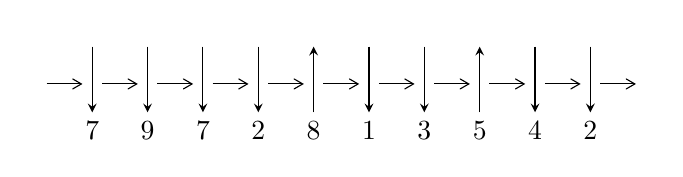
\begin{tikzpicture}[x=20pt, y=17pt]
	% nodes
	\node (C0) at (0, 0) {};
	\node (C1) at (1, 0) {};
	\node (C1U) at (1, +1) {};
	\node (C1D) at (1, -1) {7};

	\node (C2) at (2, 0) {};
	\node (C2U) at (2, +1) {};
	\node (C2D) at (2, -1) {9};

	\node (C3) at (3, 0) {};
	\node (C3U) at (3, +1) {};
	\node (C3D) at (3, -1) {7};

	\node (C4) at (4, 0) {};
	\node (C4U) at (4, +1) {};
	\node (C4D) at (4, -1) {2};

	\node (C5) at (5, 0) {};
	\node (C5U) at (5, +1) {};
	\node (C5D) at (5, -1) {8};

	\node (C6) at (6, 0) {};
	\node (C6U) at (6, +1) {};
	\node (C6D) at (6, -1) {1};

	\node (C7) at (7, 0) {};
	\node (C7U) at (7, +1) {};
	\node (C7D) at (7, -1) {3};

	\node (C8) at (8, 0) {};
	\node (C8U) at (8, +1) {};
	\node (C8D) at (8, -1) {5};

	\node (C9) at (9, 0) {};
	\node (C9U) at (9, +1) {};
	\node (C9D) at (9, -1) {4};

	\node (C10) at (10, 0) {};
	\node (C10U) at (10, +1) {};
	\node (C10D) at (10, -1) {2};
	\node (C11) at (11, 0) {};

	% arrows
	\draw[->,>={angle 60}]
	(C0) edge (C1) (C1) edge (C2) (C2) edge (C3) (C3) edge (C4) (C4) edge (C5) (C5) edge (C6) (C6) edge (C7) (C7) edge (C8) (C8) edge (C9) (C9) edge (C10) (C10) edge (C11) ;	\draw[->,>=stealth]
	(C1U) edge (C1D) (C2U) edge (C2D) (C3U) edge (C3D) (C4U) edge (C4D) (C5D) edge (C5U) (C6U) edge (C6D) (C7U) edge (C7D) (C8D) edge (C8U) (C9U) edge (C9D) (C10U) edge (C10D) ;
	\end{tikzpicture} \\
\hhline{~~} \\& 
\textbf{Solving Sequence} \\ \cline{2-2} 
 &
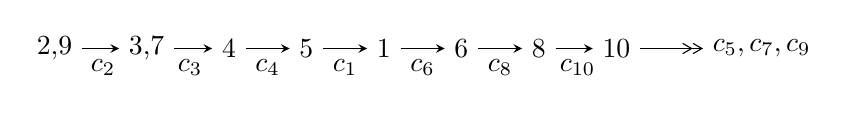
\begin{tikzpicture}[x=28pt, y=7pt]
	% node
	\node (A0) at (-1/8, 0) {2,9};
	\node (A1) at (17/16, 0) {3,7};
	\node (A2) at (17/8, 0) {4};
	\node (A3) at (25/8, 0) {5};
	\node (A4) at (33/8, 0) {1};
	\node (A5) at (41/8, 0) {6};
	\node (A6) at (49/8, 0) {8};
	\node (A7) at (57/8, 0) {10};
	\node (C1) at (1/2, -1) {$c_{2}$};
	\node (C2) at (13/8, -1) {$c_{3}$};
	\node (C3) at (21/8, -1) {$c_{4}$};
	\node (C4) at (29/8, -1) {$c_{1}$};
	\node (C5) at (37/8, -1) {$c_{6}$};
	\node (C6) at (45/8, -1) {$c_{8}$};
	\node (C7) at (53/8, -1) {$c_{10}$};
	\node (A8) at (9, 0) {$c_{5},c_{7},c_{9}$};

	% edge
	\draw[->,>=stealth]	
	(A0) edge (A1) (A1) edge (A2) (A2) edge (A3) (A3) edge (A4) (A4) edge (A5) (A5) edge (A6) (A6) edge (A7) ;
	\draw[->>,>={angle 60}]	
	(A7) edge (A8);
\end{tikzpicture} \\ 

\end{tabular} \\

\footnotetext{
The image of knot diagram is generated by the software ``\textbf{Draw programme}" developed by Andrew Bartholomew(\url{http://www.layer8.co.uk/maths/draw/index.htm\#Running-draw}), where we modified some parts for our purpose(\url{https://github.com/CATsTAILs/LinksPainter}).
}\phantom \\ \newline 
\centering \textbf{Ideals for irreducible components\footnotemark of $X_{\text{par}}$} 
 
\begin{align*}
I^u_{1}&=\langle 
u^6-2 u^5+3 u^4-2 u^3+3 u^2+b-1,\;- u^8+3 u^7-5 u^6+4 u^5-4 u^4+2 u^3+u^2+2 a-4 u-1,\\
\phantom{I^u_{1}}&\phantom{= \langle  }u^9-5 u^8+13 u^7-20 u^6+22 u^5-18 u^4+11 u^3-5 u+2\rangle \\
I^u_{2}&=\langle 
u^2+b+u+1,\;u^3+2 u^2+a+2 u+2,\;u^5+2 u^4+3 u^3+2 u^2-1\rangle \\
I^u_{3}&=\langle 
- u^2 a+b-1,\;a^2+2 a u-2 u^2+3 a-3 u-2,\;u^3+u^2-1\rangle \\
\\
\end{align*}
\raggedright * 3 irreducible components of $\dim_{\mathbb{C}}=0$, with total 20 representations.\\
\footnotetext{All coefficients of polynomials are rational numbers. But the coefficients are sometimes approximated in decimal forms when there is not enough margin.}
\newpage
\renewcommand{\arraystretch}{1}
\centering \section*{I. $I^u_{1}= \langle u^6-2 u^5+3 u^4-2 u^3+3 u^2+b-1,\;- u^8+3 u^7+\cdots+2 a-1,\;u^9-5 u^8+\cdots-5 u+2 \rangle$}
\flushleft \textbf{(i) Arc colorings}\\
\begin{tabular}{m{7pt} m{180pt} m{7pt} m{180pt} }
\flushright $a_{2}=$&$\begin{pmatrix}1\\0\end{pmatrix}$ \\
\flushright $a_{9}=$&$\begin{pmatrix}0\\u\end{pmatrix}$ \\
\flushright $a_{3}=$&$\begin{pmatrix}1\\u^2\end{pmatrix}$ \\
\flushright $a_{7}=$&$\begin{pmatrix}\frac{1}{2} u^8-\frac{3}{2} u^7+\cdots+2 u+\frac{1}{2}\\- u^6+2 u^5-3 u^4+2 u^3-3 u^2+1\end{pmatrix}$ \\
\flushright $a_{4}=$&$\begin{pmatrix}-\frac{5}{2} u^8+\frac{21}{2} u^7+\cdots-8 u+\frac{13}{2}\\u^6-2 u^5+3 u^4-2 u^3+3 u^2-1\end{pmatrix}$ \\
\flushright $a_{5}=$&$\begin{pmatrix}-\frac{5}{2} u^8+\frac{21}{2} u^7+\cdots-8 u+\frac{15}{2}\\u^6-2 u^5+3 u^4-2 u^3+3 u^2-1\end{pmatrix}$ \\
\flushright $a_{1}=$&$\begin{pmatrix}\frac{1}{2} u^8-\frac{5}{2} u^7+\cdots+2 u-\frac{3}{2}\\u^7-3 u^6+5 u^5-4 u^4+4 u^3-2 u^2- u+1\end{pmatrix}$ \\
\flushright $a_{6}=$&$\begin{pmatrix}- u^8+4 u^7-9 u^6+12 u^5-12 u^4+9 u^3-4 u^2- u+3\\-2 u^8+9 u^7-19 u^6+24 u^5-22 u^4+17 u^3-6 u^2-6 u+4\end{pmatrix}$ \\
\flushright $a_{8}=$&$\begin{pmatrix}\frac{3}{2} u^8-\frac{13}{2} u^7+\cdots+6 u-\frac{5}{2}\\- u^8+4 u^7-8 u^6+9 u^5-8 u^4+6 u^3- u^2-2 u+1\end{pmatrix}$ \\
\flushright $a_{10}=$&$\begin{pmatrix}\frac{1}{2} u^8-\frac{3}{2} u^7+\cdots+u-\frac{1}{2}\\u^7-3 u^6+5 u^5-4 u^4+4 u^3-2 u^2- u+1\end{pmatrix}$\\&\end{tabular}
\flushleft \textbf{(ii) Obstruction class $= -1$}\\~\\
\flushleft \textbf{(iii) Cusp Shapes $= u^8-5 u^7+12 u^6-15 u^5+12 u^4-4 u^3+8 u-10$}\\~\\
\newpage\renewcommand{\arraystretch}{1}
\flushleft \textbf{(iv) u-Polynomials at the component}\newline \\
\begin{tabular}{m{50pt}|m{274pt}}
Crossings & \hspace{64pt}u-Polynomials at each crossing \\
\hline $$\begin{aligned}c_{1},c_{4},c_{6}\end{aligned}$$&$\begin{aligned}
&u^9- u^8-7 u^7+7 u^6+13 u^5-13 u^4+2 u^3+u^2+1
\end{aligned}$\\
\hline $$\begin{aligned}c_{2}\end{aligned}$$&$\begin{aligned}
&u^9-5 u^8+13 u^7-20 u^6+22 u^5-18 u^4+11 u^3-5 u+2
\end{aligned}$\\
\hline $$\begin{aligned}c_{3},c_{7}\end{aligned}$$&$\begin{aligned}
&u^9+7 u^8+26 u^7+61 u^6+103 u^5+129 u^4+125 u^3+86 u^2+40 u+8
\end{aligned}$\\
\hline $$\begin{aligned}c_{5},c_{8}\end{aligned}$$&$\begin{aligned}
&u^9+6 u^7-3 u^6+14 u^5-10 u^4+13 u^3-7 u^2- u+1
\end{aligned}$\\
\hline $$\begin{aligned}c_{9}\end{aligned}$$&$\begin{aligned}
&u^9-11 u^7+2 u^6+35 u^5-32 u^4+47 u^3+8 u^2+u+13
\end{aligned}$\\
\hline $$\begin{aligned}c_{10}\end{aligned}$$&$\begin{aligned}
&u^9+15 u^8+89 u^7+253 u^6+325 u^5+129 u^4+16 u^3-25 u^2-2 u+1
\end{aligned}$\\
\hline
\end{tabular}\\~\\
\newpage\renewcommand{\arraystretch}{1}
\flushleft \textbf{(v) Riley Polynomials at the component}\newline \\
\begin{tabular}{m{50pt}|m{274pt}}
Crossings & \hspace{64pt}Riley Polynomials at each crossing \\
\hline $$\begin{aligned}c_{1},c_{4},c_{6}\end{aligned}$$&$\begin{aligned}
&y^9-15 y^8+89 y^7-253 y^6+325 y^5-129 y^4+16 y^3+25 y^2-2 y-1
\end{aligned}$\\
\hline $$\begin{aligned}c_{2}\end{aligned}$$&$\begin{aligned}
&y^9+y^8+13 y^7+14 y^6+40 y^5+50 y^4-19 y^3-38 y^2+25 y-4
\end{aligned}$\\
\hline $$\begin{aligned}c_{3},c_{7}\end{aligned}$$&$\begin{aligned}
&y^9+3 y^8+\cdots+224 y-64
\end{aligned}$\\
\hline $$\begin{aligned}c_{5},c_{8}\end{aligned}$$&$\begin{aligned}
&y^9+12 y^8+64 y^7+185 y^6+290 y^5+210 y^4+7 y^3-55 y^2+15 y-1
\end{aligned}$\\
\hline $$\begin{aligned}c_{9}\end{aligned}$$&$\begin{aligned}
&y^9-22 y^8+\cdots-207 y-169
\end{aligned}$\\
\hline $$\begin{aligned}c_{10}\end{aligned}$$&$\begin{aligned}
&y^9-47 y^8+\cdots+54 y-1
\end{aligned}$\\
\hline
\end{tabular}\\~\\
\newpage\flushleft \textbf{(vi) Complex Volumes and Cusp Shapes}
$$\begin{array}{c|c|c}  
\text{Solutions to }I^u_{1}& \I (\text{vol} + \sqrt{-1}CS) & \text{Cusp shape}\\
 \hline 
\begin{aligned}
u &= -0.204797 + 1.087900 I \\
a &= -0.055258 + 1.397040 I \\
b &= \phantom{-}0.689596 - 0.376245 I\end{aligned}
 & \phantom{-}2.64060 + 1.65275 I & -0.59079 - 4.28210 I \\ \hline\begin{aligned}
u &= -0.204797 - 1.087900 I \\
a &= -0.055258 - 1.397040 I \\
b &= \phantom{-}0.689596 + 0.376245 I\end{aligned}
 & \phantom{-}2.64060 - 1.65275 I & -0.59079 + 4.28210 I \\ \hline\begin{aligned}
u &= \phantom{-}0.647333 + 0.135453 I \\
a &= \phantom{-}1.54477 + 0.21297 I \\
b &= -0.017613 - 0.474078 I\end{aligned}
 & -0.87559 - 2.35950 I & -4.89060 + 1.18144 I \\ \hline\begin{aligned}
u &= \phantom{-}0.647333 - 0.135453 I \\
a &= \phantom{-}1.54477 - 0.21297 I \\
b &= -0.017613 + 0.474078 I\end{aligned}
 & -0.87559 + 2.35950 I & -4.89060 - 1.18144 I \\ \hline\begin{aligned}
u &= -0.531326\phantom{ +0.000000I} \\
a &= -0.232368\phantom{ +0.000000I} \\
b &= -0.493195\phantom{ +0.000000I}\end{aligned}
 & -0.846327\phantom{ +0.000000I} & -11.7230\phantom{ +0.000000I} \\ \hline\begin{aligned}
u &= \phantom{-}1.20035 + 1.05816 I \\
a &= \phantom{-}0.77288 - 1.22009 I \\
b &= \phantom{-}1.96815 + 0.34791 I\end{aligned}
 & -14.0726 - 9.2039 I & -9.16258 + 4.28229 I \\ \hline\begin{aligned}
u &= \phantom{-}1.20035 - 1.05816 I \\
a &= \phantom{-}0.77288 + 1.22009 I \\
b &= \phantom{-}1.96815 - 0.34791 I\end{aligned}
 & -14.0726 + 9.2039 I & -9.16258 - 4.28229 I \\ \hline\begin{aligned}
u &= \phantom{-}1.12278 + 1.21739 I \\
a &= -0.396214 + 0.245006 I \\
b &= -1.89353 + 0.26305 I\end{aligned}
 & -13.58820 + 0.68871 I & -9.49454 - 0.10018 I \\ \hline\begin{aligned}
u &= \phantom{-}1.12278 - 1.21739 I \\
a &= -0.396214 - 0.245006 I \\
b &= -1.89353 - 0.26305 I\end{aligned}
 & -13.58820 - 0.68871 I & -9.49454 + 0.10018 I\\
 \hline 
 \end{array}$$\newpage\newpage\renewcommand{\arraystretch}{1}
\centering \section*{II. $I^u_{2}= \langle u^2+b+u+1,\;u^3+2 u^2+a+2 u+2,\;u^5+2 u^4+3 u^3+2 u^2-1 \rangle$}
\flushleft \textbf{(i) Arc colorings}\\
\begin{tabular}{m{7pt} m{180pt} m{7pt} m{180pt} }
\flushright $a_{2}=$&$\begin{pmatrix}1\\0\end{pmatrix}$ \\
\flushright $a_{9}=$&$\begin{pmatrix}0\\u\end{pmatrix}$ \\
\flushright $a_{3}=$&$\begin{pmatrix}1\\u^2\end{pmatrix}$ \\
\flushright $a_{7}=$&$\begin{pmatrix}- u^3-2 u^2-2 u-2\\- u^2- u-1\end{pmatrix}$ \\
\flushright $a_{4}=$&$\begin{pmatrix}u^3+2 u^2+3 u+2\\u^2+u+1\end{pmatrix}$ \\
\flushright $a_{5}=$&$\begin{pmatrix}u^3+u^2+2 u+1\\u^2+u+1\end{pmatrix}$ \\
\flushright $a_{1}=$&$\begin{pmatrix}- u^4-2 u^3-4 u^2-4 u-2\\- u^4-2 u^3-3 u^2-2 u-1\end{pmatrix}$ \\
\flushright $a_{6}=$&$\begin{pmatrix}2 u^4+4 u^3+6 u^2+5 u+1\\u^4+2 u^3+3 u^2+3 u+1\end{pmatrix}$ \\
\flushright $a_{8}=$&$\begin{pmatrix}- u^2- u-2\\- u^4-2 u^3-3 u^2- u\end{pmatrix}$ \\
\flushright $a_{10}=$&$\begin{pmatrix}-2 u^4-4 u^3-7 u^2-6 u-3\\- u^4-2 u^3-3 u^2-2 u-1\end{pmatrix}$\\&\end{tabular}
\flushleft \textbf{(ii) Obstruction class $= 1$}\\~\\
\flushleft \textbf{(iii) Cusp Shapes $= 3 u^4+3 u^3+7 u^2+u-8$}\\~\\
\newpage\renewcommand{\arraystretch}{1}
\flushleft \textbf{(iv) u-Polynomials at the component}\newline \\
\begin{tabular}{m{50pt}|m{274pt}}
Crossings & \hspace{64pt}u-Polynomials at each crossing \\
\hline $$\begin{aligned}c_{1},c_{4}\end{aligned}$$&$\begin{aligned}
&u^5+u^4-2 u^3- u^2+u+1
\end{aligned}$\\
\hline $$\begin{aligned}c_{2}\end{aligned}$$&$\begin{aligned}
&u^5+2 u^4+3 u^3+2 u^2-1
\end{aligned}$\\
\hline $$\begin{aligned}c_{3}\end{aligned}$$&$\begin{aligned}
&u^5+2 u^3+u^2+1
\end{aligned}$\\
\hline $$\begin{aligned}c_{5}\end{aligned}$$&$\begin{aligned}
&u^5+u^3-2 u^2-1
\end{aligned}$\\
\hline $$\begin{aligned}c_{6}\end{aligned}$$&$\begin{aligned}
&u^5- u^4-2 u^3+u^2+u-1
\end{aligned}$\\
\hline $$\begin{aligned}c_{7}\end{aligned}$$&$\begin{aligned}
&u^5+2 u^3- u^2-1
\end{aligned}$\\
\hline $$\begin{aligned}c_{8}\end{aligned}$$&$\begin{aligned}
&u^5+u^3+2 u^2+1
\end{aligned}$\\
\hline $$\begin{aligned}c_{9}\end{aligned}$$&$\begin{aligned}
&u^5-2 u^3+3 u^2-2 u+1
\end{aligned}$\\
\hline $$\begin{aligned}c_{10}\end{aligned}$$&$\begin{aligned}
&u^5-5 u^4+8 u^3-7 u^2+3 u-1
\end{aligned}$\\
\hline
\end{tabular}\\~\\
\newpage\renewcommand{\arraystretch}{1}
\flushleft \textbf{(v) Riley Polynomials at the component}\newline \\
\begin{tabular}{m{50pt}|m{274pt}}
Crossings & \hspace{64pt}Riley Polynomials at each crossing \\
\hline $$\begin{aligned}c_{1},c_{4},c_{6}\end{aligned}$$&$\begin{aligned}
&y^5-5 y^4+8 y^3-7 y^2+3 y-1
\end{aligned}$\\
\hline $$\begin{aligned}c_{2}\end{aligned}$$&$\begin{aligned}
&y^5+2 y^4+y^3+4 y-1
\end{aligned}$\\
\hline $$\begin{aligned}c_{3},c_{7}\end{aligned}$$&$\begin{aligned}
&y^5+4 y^4+4 y^3- y^2-2 y-1
\end{aligned}$\\
\hline $$\begin{aligned}c_{5},c_{8}\end{aligned}$$&$\begin{aligned}
&y^5+2 y^4+y^3-4 y^2-4 y-1
\end{aligned}$\\
\hline $$\begin{aligned}c_{9}\end{aligned}$$&$\begin{aligned}
&y^5-4 y^4- y^2-2 y-1
\end{aligned}$\\
\hline $$\begin{aligned}c_{10}\end{aligned}$$&$\begin{aligned}
&y^5-9 y^4-11 y^2-5 y-1
\end{aligned}$\\
\hline
\end{tabular}\\~\\
\newpage\flushleft \textbf{(vi) Complex Volumes and Cusp Shapes}
$$\begin{array}{c|c|c}  
\text{Solutions to }I^u_{2}& \I (\text{vol} + \sqrt{-1}CS) & \text{Cusp shape}\\
 \hline 
\begin{aligned}
u &= -0.885210 + 0.546617 I \\
a &= -1.299020 - 0.279409 I \\
b &= -0.599596 + 0.421125 I\end{aligned}
 & -1.44657 + 3.45949 I & -7.29654 - 5.67761 I \\ \hline\begin{aligned}
u &= -0.885210 - 0.546617 I \\
a &= -1.299020 + 0.279409 I \\
b &= -0.599596 - 0.421125 I\end{aligned}
 & -1.44657 - 3.45949 I & -7.29654 + 5.67761 I \\ \hline\begin{aligned}
u &= -0.361950 + 1.318330 I \\
a &= \phantom{-}0.098088 + 1.045130 I \\
b &= \phantom{-}0.968932 - 0.363992 I\end{aligned}
 & \phantom{-}1.57933 + 1.42206 I & -9.07660 - 1.47974 I \\ \hline\begin{aligned}
u &= -0.361950 - 1.318330 I \\
a &= \phantom{-}0.098088 - 1.045130 I \\
b &= \phantom{-}0.968932 + 0.363992 I\end{aligned}
 & \phantom{-}1.57933 - 1.42206 I & -9.07660 + 1.47974 I \\ \hline\begin{aligned}
u &= \phantom{-}0.494320\phantom{ +0.000000I} \\
a &= -3.59813\phantom{ +0.000000I} \\
b &= -1.73867\phantom{ +0.000000I}\end{aligned}
 & -6.84525\phantom{ +0.000000I} & -5.25370\phantom{ +0.000000I}\\
 \hline 
 \end{array}$$\newpage\newpage\renewcommand{\arraystretch}{1}
\centering \section*{III. $I^u_{3}= \langle - u^2 a+b-1,\;a^2+2 a u-2 u^2+3 a-3 u-2,\;u^3+u^2-1 \rangle$}
\flushleft \textbf{(i) Arc colorings}\\
\begin{tabular}{m{7pt} m{180pt} m{7pt} m{180pt} }
\flushright $a_{2}=$&$\begin{pmatrix}1\\0\end{pmatrix}$ \\
\flushright $a_{9}=$&$\begin{pmatrix}0\\u\end{pmatrix}$ \\
\flushright $a_{3}=$&$\begin{pmatrix}1\\u^2\end{pmatrix}$ \\
\flushright $a_{7}=$&$\begin{pmatrix}a\\u^2 a+1\end{pmatrix}$ \\
\flushright $a_{4}=$&$\begin{pmatrix}a+1\\u^2 a+u^2+1\end{pmatrix}$ \\
\flushright $a_{5}=$&$\begin{pmatrix}- u^2 a- u^2+a\\u^2 a+u^2+1\end{pmatrix}$ \\
\flushright $a_{1}=$&$\begin{pmatrix}u^2 a- u^2+a-2 u\\u^2 a+a u- a- u-2\end{pmatrix}$ \\
\flushright $a_{6}=$&$\begin{pmatrix}-2 u^2 a-2 a u+u+2\\-2 a u- u\end{pmatrix}$ \\
\flushright $a_{8}=$&$\begin{pmatrix}a-1\\u^2 a- u^2+1\end{pmatrix}$ \\
\flushright $a_{10}=$&$\begin{pmatrix}2 u^2 a+a u- u^2-3 u-2\\u^2 a+a u- a- u-2\end{pmatrix}$\\&\end{tabular}
\flushleft \textbf{(ii) Obstruction class $= -1$}\\~\\
\flushleft \textbf{(iii) Cusp Shapes $= -4 u-14$}\\~\\
\newpage\renewcommand{\arraystretch}{1}
\flushleft \textbf{(iv) u-Polynomials at the component}\newline \\
\begin{tabular}{m{50pt}|m{274pt}}
Crossings & \hspace{64pt}u-Polynomials at each crossing \\
\hline $$\begin{aligned}c_{1},c_{4},c_{6}\end{aligned}$$&$\begin{aligned}
&u^6+u^5-4 u^4-4 u^3+4 u^2+8 u-7
\end{aligned}$\\
\hline $$\begin{aligned}c_{2}\end{aligned}$$&$\begin{aligned}
&(u^3+u^2-1)^2
\end{aligned}$\\
\hline $$\begin{aligned}c_{3},c_{7}\end{aligned}$$&$\begin{aligned}
&(u-1)^6
\end{aligned}$\\
\hline $$\begin{aligned}c_{5},c_{8}\end{aligned}$$&$\begin{aligned}
&u^6+3 u^5+6 u^4+12 u^3+10 u^2+10 u+1
\end{aligned}$\\
\hline $$\begin{aligned}c_{9}\end{aligned}$$&$\begin{aligned}
&u^6+u^5-6 u^4+8 u^3+2 u^2-6 u-11
\end{aligned}$\\
\hline $$\begin{aligned}c_{10}\end{aligned}$$&$\begin{aligned}
&u^6+9 u^5+32 u^4+78 u^3+136 u^2+120 u+49
\end{aligned}$\\
\hline
\end{tabular}\\~\\
\newpage\renewcommand{\arraystretch}{1}
\flushleft \textbf{(v) Riley Polynomials at the component}\newline \\
\begin{tabular}{m{50pt}|m{274pt}}
Crossings & \hspace{64pt}Riley Polynomials at each crossing \\
\hline $$\begin{aligned}c_{1},c_{4},c_{6}\end{aligned}$$&$\begin{aligned}
&y^6-9 y^5+32 y^4-78 y^3+136 y^2-120 y+49
\end{aligned}$\\
\hline $$\begin{aligned}c_{2}\end{aligned}$$&$\begin{aligned}
&(y^3- y^2+2 y-1)^2
\end{aligned}$\\
\hline $$\begin{aligned}c_{3},c_{7}\end{aligned}$$&$\begin{aligned}
&(y-1)^6
\end{aligned}$\\
\hline $$\begin{aligned}c_{5},c_{8}\end{aligned}$$&$\begin{aligned}
&y^6+3 y^5-16 y^4-82 y^3-128 y^2-80 y+1
\end{aligned}$\\
\hline $$\begin{aligned}c_{9}\end{aligned}$$&$\begin{aligned}
&y^6-13 y^5+24 y^4-98 y^3+232 y^2-80 y+121
\end{aligned}$\\
\hline $$\begin{aligned}c_{10}\end{aligned}$$&$\begin{aligned}
&y^6-17 y^5-108 y^4+558 y^3+2912 y^2-1072 y+2401
\end{aligned}$\\
\hline
\end{tabular}\\~\\
\newpage\flushleft \textbf{(vi) Complex Volumes and Cusp Shapes}
$$\begin{array}{c|c|c}  
\text{Solutions to }I^u_{3}& \I (\text{vol} + \sqrt{-1}CS) & \text{Cusp shape}\\
 \hline 
\begin{aligned}
u &= -0.877439 + 0.744862 I \\
a &= -0.240939 - 0.027206 I \\
b &= \phantom{-}0.912616 + 0.309089 I\end{aligned}
 & -3.55561 + 2.82812 I & -10.49024 - 2.97945 I \\ \hline\begin{aligned}
u &= -0.877439 + 0.744862 I \\
a &= -1.00418 - 1.46252 I \\
b &= -1.12770 + 0.99805 I\end{aligned}
 & -3.55561 + 2.82812 I & -10.49024 - 2.97945 I \\ \hline\begin{aligned}
u &= -0.877439 - 0.744862 I \\
a &= -0.240939 + 0.027206 I \\
b &= \phantom{-}0.912616 - 0.309089 I\end{aligned}
 & -3.55561 - 2.82812 I & -10.49024 + 2.97945 I \\ \hline\begin{aligned}
u &= -0.877439 - 0.744862 I \\
a &= -1.00418 + 1.46252 I \\
b &= -1.12770 - 0.99805 I\end{aligned}
 & -3.55561 - 2.82812 I & -10.49024 + 2.97945 I \\ \hline\begin{aligned}
u &= \phantom{-}0.754878\phantom{ +0.000000I} \\
a &= \phantom{-}0.983762\phantom{ +0.000000I} \\
b &= \phantom{-}1.56059\phantom{ +0.000000I}\end{aligned}
 & -7.69319\phantom{ +0.000000I} & -17.0200\phantom{ +0.000000I} \\ \hline\begin{aligned}
u &= \phantom{-}0.754878\phantom{ +0.000000I} \\
a &= -5.49352\phantom{ +0.000000I} \\
b &= -2.13043\phantom{ +0.000000I}\end{aligned}
 & -7.69319\phantom{ +0.000000I} & -17.0200\phantom{ +0.000000I}\\
 \hline 
 \end{array}$$\newpage
\newpage\renewcommand{\arraystretch}{1}
\centering \section*{ IV. u-Polynomials}
\begin{tabular}{m{50pt}|m{274pt}}
Crossings & \hspace{64pt}u-Polynomials at each crossing \\
\hline $$\begin{aligned}c_{1},c_{4}\end{aligned}$$&$\begin{aligned}
&(u^5+u^4-2 u^3- u^2+u+1)(u^6+u^5-4 u^4-4 u^3+4 u^2+8 u-7)\\
&\cdot(u^9- u^8-7 u^7+7 u^6+13 u^5-13 u^4+2 u^3+u^2+1)
\end{aligned}$\\
\hline $$\begin{aligned}c_{2}\end{aligned}$$&$\begin{aligned}
&(u^3+u^2-1)^2(u^5+2 u^4+3 u^3+2 u^2-1)\\
&\cdot(u^9-5 u^8+13 u^7-20 u^6+22 u^5-18 u^4+11 u^3-5 u+2)
\end{aligned}$\\
\hline $$\begin{aligned}c_{3}\end{aligned}$$&$\begin{aligned}
&(u-1)^6(u^5+2 u^3+u^2+1)\\
&\cdot(u^9+7 u^8+26 u^7+61 u^6+103 u^5+129 u^4+125 u^3+86 u^2+40 u+8)
\end{aligned}$\\
\hline $$\begin{aligned}c_{5}\end{aligned}$$&$\begin{aligned}
&(u^5+u^3-2 u^2-1)(u^6+3 u^5+6 u^4+12 u^3+10 u^2+10 u+1)\\
&\cdot(u^9+6 u^7-3 u^6+14 u^5-10 u^4+13 u^3-7 u^2- u+1)
\end{aligned}$\\
\hline $$\begin{aligned}c_{6}\end{aligned}$$&$\begin{aligned}
&(u^5- u^4-2 u^3+u^2+u-1)(u^6+u^5-4 u^4-4 u^3+4 u^2+8 u-7)\\
&\cdot(u^9- u^8-7 u^7+7 u^6+13 u^5-13 u^4+2 u^3+u^2+1)
\end{aligned}$\\
\hline $$\begin{aligned}c_{7}\end{aligned}$$&$\begin{aligned}
&(u-1)^6(u^5+2 u^3- u^2-1)\\
&\cdot(u^9+7 u^8+26 u^7+61 u^6+103 u^5+129 u^4+125 u^3+86 u^2+40 u+8)
\end{aligned}$\\
\hline $$\begin{aligned}c_{8}\end{aligned}$$&$\begin{aligned}
&(u^5+u^3+2 u^2+1)(u^6+3 u^5+6 u^4+12 u^3+10 u^2+10 u+1)\\
&\cdot(u^9+6 u^7-3 u^6+14 u^5-10 u^4+13 u^3-7 u^2- u+1)
\end{aligned}$\\
\hline $$\begin{aligned}c_{9}\end{aligned}$$&$\begin{aligned}
&(u^5-2 u^3+3 u^2-2 u+1)(u^6+u^5-6 u^4+8 u^3+2 u^2-6 u-11)\\
&\cdot(u^9-11 u^7+2 u^6+35 u^5-32 u^4+47 u^3+8 u^2+u+13)
\end{aligned}$\\
\hline $$\begin{aligned}c_{10}\end{aligned}$$&$\begin{aligned}
&(u^5-5 u^4+8 u^3-7 u^2+3 u-1)\\
&\cdot(u^6+9 u^5+32 u^4+78 u^3+136 u^2+120 u+49)\\
&\cdot(u^9+15 u^8+89 u^7+253 u^6+325 u^5+129 u^4+16 u^3-25 u^2-2 u+1)
\end{aligned}$\\
\hline
\end{tabular}\newpage\renewcommand{\arraystretch}{1}
\centering \section*{ V. Riley Polynomials}
\begin{tabular}{m{50pt}|m{274pt}}
Crossings & \hspace{64pt}Riley Polynomials at each crossing \\
\hline $$\begin{aligned}c_{1},c_{4},c_{6}\end{aligned}$$&$\begin{aligned}
&(y^5-5 y^4+8 y^3-7 y^2+3 y-1)\\
&\cdot(y^6-9 y^5+32 y^4-78 y^3+136 y^2-120 y+49)\\
&\cdot(y^9-15 y^8+89 y^7-253 y^6+325 y^5-129 y^4+16 y^3+25 y^2-2 y-1)
\end{aligned}$\\
\hline $$\begin{aligned}c_{2}\end{aligned}$$&$\begin{aligned}
&(y^3- y^2+2 y-1)^2(y^5+2 y^4+y^3+4 y-1)\\
&\cdot(y^9+y^8+13 y^7+14 y^6+40 y^5+50 y^4-19 y^3-38 y^2+25 y-4)
\end{aligned}$\\
\hline $$\begin{aligned}c_{3},c_{7}\end{aligned}$$&$\begin{aligned}
&((y-1)^6)(y^5+4 y^4+\cdots-2 y-1)(y^9+3 y^8+\cdots+224 y-64)
\end{aligned}$\\
\hline $$\begin{aligned}c_{5},c_{8}\end{aligned}$$&$\begin{aligned}
&(y^5+2 y^4+y^3-4 y^2-4 y-1)\\
&\cdot(y^6+3 y^5-16 y^4-82 y^3-128 y^2-80 y+1)\\
&\cdot(y^9+12 y^8+64 y^7+185 y^6+290 y^5+210 y^4+7 y^3-55 y^2+15 y-1)
\end{aligned}$\\
\hline $$\begin{aligned}c_{9}\end{aligned}$$&$\begin{aligned}
&(y^5-4 y^4- y^2-2 y-1)(y^6-13 y^5+\cdots-80 y+121)\\
&\cdot(y^9-22 y^8+\cdots-207 y-169)
\end{aligned}$\\
\hline $$\begin{aligned}c_{10}\end{aligned}$$&$\begin{aligned}
&(y^5-9 y^4-11 y^2-5 y-1)\\
&\cdot(y^6-17 y^5-108 y^4+558 y^3+2912 y^2-1072 y+2401)\\
&\cdot(y^9-47 y^8+\cdots+54 y-1)
\end{aligned}$\\
\hline
\end{tabular}
\vskip 2pc
\end{document}